
\chapter{绪论}\label{chap:intro}
\section{研究背景和意义}
**********************

\begin{figure}[h]
	\centering
	
\includegraphics[width=0.6\textwidth]{figures/c1fig1.jpg}
	\caption{******}    
	\label{fig:fig07}
\end{figure}

\begin{figure}[h]
	\centering
	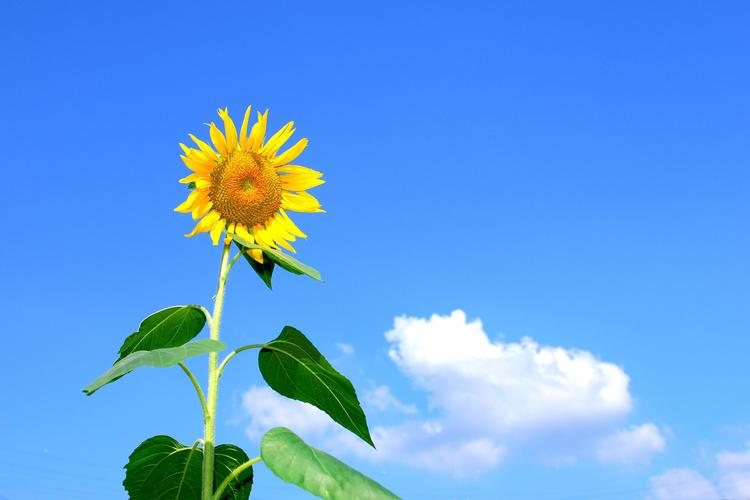
\includegraphics[width=0.6\textwidth]{figures/c1fig2.jpeg}
	\caption{******}    
	\label{fig:fig07}
\end{figure}

\section{国内外研究现状及发展趋势}
**********************




\section{论文主要内容和结构安排}
{\color{blue}河南师范大学}位于豫北名城新乡市，北依巍巍太行，南濒滔滔黄河，坐落在广袤的牧野大地、美丽的卫水之滨。学校是国家中西部高等教育振兴计划支持高校、国家“111计划”实施高校、河南省人民政府与教育部共建高校、教育部本科教学工作水平评估优秀学校和河南省特色骨干大学，\underline{河南省“双一流”创建高校}，三度蝉联全国文明单位，入选第二届全国文明校园{\color{red}\cite{R001}}。

文献{\color{red}\textcite{R002}}表明...............

\subsection{学校情况}
学校历史底蕴深厚，办学资源丰富\footnote{学校前身是始建于1923年的中州大学（原国立河南大学前身）理科和创建于1951年的平原师范学院，历经河南师范学院二院、河南第二师范学院、新乡师范学院等阶段，1985年始称河南师范大学。}。在百年的办学历程中，逐步熔铸了“厚德博学 止于至善”的校训、“明德 正学 倡和 出新”的校风、“修至学 立世范 启智慧 益品行”的教风、“尚诚朴 勤学问 重团结 养正气”的学风，积累和沉淀了“崇文明道 尚诚守德 抱朴求真”的师大精神，以校风淳、教风正、学风浓、教学水平高享誉省内外。学校占地面积139.53万平方米，建筑面积110.01万平方米，中外文纸质图书326.18余万册，电子图书1045.89余万册。建有全球唯一一家帕瓦罗蒂音乐艺术中心和河南省规模最大、种类最多的生物资源博物馆，办有附属中学、附属小学和幼儿园。

%%%   定理
\begin{thm}
	\rm{对于XXXXXXXXX，通过XXXXXXXXX可以表示为}
	\setlength\arraycolsep{1pt}   % 调整eqnarray等号两边空白
	\begin{eqnarray} 　 \label{eq3_06}   
		{{\pmb{\hat {\text g}}}_{mk}} = \sqrt {\tau {\rho _{\rm{\text p}}}} {{\pmb{\text R}}_{mk}}{{\pmb {\Xi }}_{mk}}{{\pmb{\mathord{\buildrel{\lower3pt\hbox{$\scriptscriptstyle\smile$}} \over {\text y}} }}_{mk,{\rm{\text p}}}},
	\end{eqnarray}
\end{thm}

%  证明
\begin{proof}
	根据XXXXXXXXXXX
\end{proof}

学校学科门类齐全，培养体系完备。现有哲学、经济学、法学、教育学、文学、历史学、理学、工学、农学、管理学、艺术学等11大学科门类。设有25个学院（部），4个书院，89个本科专业，其中国家一流本科专业建设点34个，省级一流本科专业建设点23个；32个硕士学位授权一级学科、21个硕士专业学位类别，10个博士学位授权一级学科、1个博士专业学位类别，7个博士后科研流动站，各类学生7.5万余人。拥有国家学科创新引智基地（“111计划”）2个、河南省特色骨干A类学科4个、河南省特需急需特色骨干学科（群）1个、河南省一级重点学科28个，化学、工程学、材料科学、环境/生态学、植物与动物科学等5个学科持续进入ESI全球前1\%，化学、地球与环境科学、物理学等3个学科持续进入本领域自然指数内地高校百强学科榜单。






\begin{table}
	\caption{\label{tab:test}不同DACs位数的量化系数} 
	\centering
	\renewcommand\arraystretch{1.2}  
	\begin{tabular}{c c c c c c}
		\hline
		{\kern 3pt}${b_m}$ & 1 & 2  & 3 & 4 &  5 {\kern 3pt}\\
		{\kern 3pt}${\alpha _m}$ & 0.6366 & 0.8825 & 0.96546 & 0.990503 &  0.997501 {\kern 3pt} \\
		\hline
	\end{tabular}
\end{table}







